\documentclass[aspectratio=169,11pt]{beamer}

% Shared style, ported from the UF Animal Sciences 2026 talk (ib-tutorials.sty at the repo root).
\makeatletter\def\input@path{{./}{../}}\makeatother
\usepackage{ib-tutorials}

\usepackage[utf8]{inputenc}
\usepackage{graphicx}
% Resolve ../pictures/... whether compiling in this folder or from the repo root.
\graphicspath{{./}{../}{2-Solid-Mechanics-Under-Construction/}}
\usepackage{amsmath}
\usepackage{amssymb}

\usepackage{tikz}
\usetikzlibrary{arrows.meta}


\title{Introduction to Tensors}
\author{Laura A. Miller}
\institute{Department of Mathematics, University of Arizona}
\date{Fluid Dynamics and IBM Theory \textbullet\ Module 2}

\begin{document}

\begin{frame}[plain,b]
\maketutorialtitle
\end{frame}

\begin{frame}{Introduction to Tensors}
    \begin{itemize}
        \item Tensors are mathematical objects that generalize scalars, vectors, and matrices. 
        \item They are essential tools for describing physical quantities that have both magnitude and multiple directions, such as stress, strain, and the moment of inertia.
        \item Tensors are represented by arrays of numbers, where the number of indices indicates the order of the tensor. 
        \begin{itemize}
            \item Scalar: 0th-order tensor (magnitude only) 
            \item Vector: 1st-order tensor (magnitude and one direction) 
            \item Second-order tensor: represented by a matrix once a basis is chosen
        \end{itemize}
    \end{itemize}
\end{frame}

\begin{frame}{Tensor Notation}
    \begin{itemize}
        \item Tensors are often represented using index notation, where subscripts indicate the components of the tensor. 
        \item For example, the components of a vector $\mathbf{v}$ can be represented as $v_i$, where $i$ can take on values 1, 2, or 3 in three-dimensional space. 
        \item Similarly, the components of a matrix $\mathbf{A}$ can be represented as $A_{ij}$, where $i$ and $j$ can each take on values 1, 2, or 3. 
    \end{itemize}
\end{frame}

\begin{frame}{Tensor Operations}
    \begin{itemize}
        \item Tensors can be added, subtracted, and multiplied by scalars, just like vectors and matrices. 
        \item They can also be multiplied together using the tensor product, which combines two tensors to form a higher-order tensor. 
        \item Other important tensor operations include the dot product and the cross product, which are generalizations of the corresponding vector operations. 
    \end{itemize}
\end{frame}

\begin{frame}{What Is a Basis?}

\begin{itemize}

    \item A \textbf{basis} is a set of linearly independent vectors that allows us
          to represent any vector or tensor in component form.
          Different bases give different component matrices, but the
          underlying geometric object does not change.

    \item The familiar \textbf{Cartesian basis}
          $\{\mathbf{e}_1,\mathbf{e}_2,\mathbf{e}_3\}$ is:
          \begin{itemize}
              \item orthonormal,
              \item fixed in space,
              \item aligned with the coordinate axes.
          \end{itemize}

    \item We often introduce a \textbf{rotated Cartesian basis}
          $\{\mathbf{m}_1,\mathbf{m}_2,\mathbf{m}_3\}$ via a rotation matrix $Q$:
          \[
              \mathbf{m}_i = \sum_{j=1}^{3} Q_{ij}\,\mathbf{e}_j, \qquad Q_{ij} = \mathbf{m}_i\cdot\mathbf{e}_j .
          \]
          The basis changes, but the physical vector or tensor does not.
          (Row $i$ of $Q$ lists the $\mathbf{e}$-components of $\mathbf{m}_i$; this is the same $Q$ used in the transformation law below. The rotation \emph{tensor} that carries each $\mathbf{e}_i$ onto $\mathbf{m}_i$ has component matrix $Q^T$.)

    \item Understanding different bases is essential for interpreting how tensors
          transform and why their component matrices change under rotation.

\end{itemize}

\end{frame}

\begin{frame}{Other Common Bases in Mechanics}

\begin{itemize}

    \item Not all bases are orthonormal or fixed.
          In many physical problems, \textbf{curvilinear bases} arise naturally.

    \item \textbf{Cylindrical basis}:
          \[
              \{\mathbf{e}_r, \mathbf{e}_\theta, \mathbf{e}_z\}
          \]
          Useful in pipes, rotating machinery, and axisymmetric geometry.
          Basis vectors vary with position.

    \item \textbf{Spherical basis}:
          \[
              \{\mathbf{e}_r, \mathbf{e}_\theta, \mathbf{e}_\phi\}
          \]
          Arises in pressure vessels, planetary models, and radially symmetric systems.

    \item \textbf{Oblique or skew bases}:
          Basis vectors are not orthogonal.
          Common in crystal mechanics and finite element methods.

    \item In each case, tensor components look different,
          but the tensor itself is unchanged.
          This is exactly why the \textbf{tensor transformation law} matters.

\end{itemize}

\end{frame}


\begin{frame}{Tensor Transformation Law (Layman’s Definition)}

\textbf{Big Idea:}  
A tensor is a physical or geometric object that does \emph{not} depend on how we choose
to describe it.  
Only its \emph{components} change when we change our point of view.

\medskip

\textbf{What changes?}  
\begin{itemize}
    \item When we rotate or change our coordinate system, the numbers in a tensor's
          matrix may look different.
    \item But the underlying object—the stretching, rotating, or mapping it represents—stays the same.
\end{itemize}

\medskip

\textbf{Tensor Transformation Law (in words):}  
\begin{quote}
When we change coordinates, a tensor automatically adjusts its components in just the
right way so that it still describes the same physical or geometric process.
\end{quote}

\end{frame}

\begin{frame}{Why the Transformation Law Matters}

\textbf{Why this matters:}
\begin{itemize}
    \item A true tensor gives the same prediction no matter what coordinate system we use.
    \item This is how we know the stress tensor, strain tensor, and deformation gradient
          describe real physical things—not artifacts of our notation.
\end{itemize}

\end{frame}


\begin{frame}{Tensor Transformation Law}

Let $\{ \mathbf{e}_1, \mathbf{e}_2, \mathbf{e}_3 \}$ and 
$\{ \mathbf{m}_1, \mathbf{m}_2, \mathbf{m}_3 \}$ be two Cartesian bases.
Let $Q$ be the orthogonal transformation matrix whose components are
\[
Q_{ij} = \mathbf{m}_i \cdot \mathbf{e}_j .
\]

\medskip
If $S$ is a second-order tensor with components $S_{ij}$ in the 
$\mathbf{e}$-basis, then its components in the 
$\mathbf{m}$-basis are given by the \textbf{tensor transformation law}:
\begin{gather*}
S^{(m)} = Q\, S^{(e)}\, Q^{T}.
\\
S^{(m)}_{ij}
=
Q_{ik}\, S^{(e)}_{kl}\, Q_{jl}.
\end{gather*}

\medskip
\begin{itemize}
\item This ensures that $S$ represents the \emph{same linear map}, even when the basis changes.
\item Scalars (0th order) remain unchanged; vectors (1st order) transform as $v^{(m)} = Q v^{(e)}$;  
  tensors (2nd order) transform with \emph{two} factors of $Q$.
\end{itemize}

\end{frame}

\begin{frame}{Matrix Representation of a Tensor -- Part 1}

\begin{itemize}

\item To compute with tensors, we express them in components relative to a basis,
just like vectors.

\item Consider the displacement gradient \(\nabla \mathbf{u}\) of a vector field
\(\mathbf{u}(x_1,x_2,x_3)\).  
It is the linear map defined by
\[
d\mathbf{u} = (\nabla \mathbf{u})\, d\mathbf{x}.
\]

\item Let \(\{ \mathbf{e}_1,\mathbf{e}_2,\mathbf{e}_3 \}\) be a Cartesian basis.
We now express both \(d\mathbf{u}\) and \(d\mathbf{x}\) in components relative to this basis.

\end{itemize}

\end{frame}


\begin{frame}{Matrix Representation of a Tensor -- Part 2}

\begin{columns}[T,onlytextwidth]
\begin{column}{0.50\textwidth}
\begin{itemize}

\item Using the component forms of \(d\mathbf{u}\) and \(d\mathbf{x}\),
the definition
\[
d\mathbf{u} = (\nabla \mathbf{u})\, d\mathbf{x}
\]
gives
\begin{align*}
du_1 &= \frac{\partial u_1}{\partial x_1} dx_1
     + \frac{\partial u_1}{\partial x_2} dx_2
     + \frac{\partial u_1}{\partial x_3} dx_3, \\
du_2 &= \frac{\partial u_2}{\partial x_1} dx_1
     + \frac{\partial u_2}{\partial x_2} dx_2
     + \frac{\partial u_2}{\partial x_3} dx_3, \\
du_3 &= \frac{\partial u_3}{\partial x_1} dx_1
     + \frac{\partial u_3}{\partial x_2} dx_2
     + \frac{\partial u_3}{\partial x_3} dx_3.
\end{align*}

\end{itemize}
\end{column}
\begin{column}{0.48\textwidth}
\begin{itemize}

\item Written in matrix form:
\[
\begin{bmatrix}
du_1 \\ du_2 \\ du_3
\end{bmatrix}
=
\begin{bmatrix}
\frac{\partial u_1}{\partial x_1} &
\frac{\partial u_1}{\partial x_2} &
\frac{\partial u_1}{\partial x_3} \\[6pt]
\frac{\partial u_2}{\partial x_1} &
\frac{\partial u_2}{\partial x_2} &
\frac{\partial u_2}{\partial x_3} \\[6pt]
\frac{\partial u_3}{\partial x_1} &
\frac{\partial u_3}{\partial x_2} &
\frac{\partial u_3}{\partial x_3}
\end{bmatrix}
\begin{bmatrix}
dx_1 \\ dx_2 \\ dx_3
\end{bmatrix}.
\]

\end{itemize}
\end{column}
\end{columns}

\end{frame}


\begin{frame}{Matrix Representation of a Tensor -- Part 3}

\begin{itemize}

\item The displacement gradient \(\nabla \mathbf{u}\) is therefore represented by
a \(3\times 3\) matrix whose entries are
\[
(\nabla \mathbf{u})_{ij} = \frac{\partial u_i}{\partial x_j}.
\]

\item Every second-order tensor can be represented this way.  
A general tensor \(S\) has components
\[
S =
\begin{bmatrix}
S_{11} & S_{12} & S_{13} \\
S_{21} & S_{22} & S_{23} \\
S_{31} & S_{32} & S_{33}
\end{bmatrix}.
\]

\item Because it behaves like a linear map, we may perform all standard
matrix operations: addition, multiplication, transpose, inverse, determinant, etc.

\end{itemize}

\end{frame}


\begin{frame}{Matrix Representation of a Tensor -- Part 4}

\begin{itemize}

\item One may compute eigenvalues, eigenvectors, tensor square roots, exponentials,
and other matrix functions using the component matrix.

\item The components \(S_{ij}\) depend on the chosen basis.  
Changing the basis changes the component matrix.

\item However, the tensor itself --- the underlying linear map --- is basis independent.

\item Thus, if
\[
\mathbf{v} = S\,\mathbf{u},
\]
then this relation holds in \emph{every} coordinate system, even though the
matrix representation of \(S\), \(\mathbf{u}\), and \(\mathbf{v}\) may change.

\end{itemize}

\end{frame}

\begin{frame}{Example: The Gradient of a Vector Field (recap)}

{\footnotesize\color{DarkGray}Recap of Parts 1--3, stated for a general vector field $\mathbf{u}$ (not only a displacement).\par}

Let $\mathbf{u}(\mathbf{x})$ be a vector field in $\mathbb{R}^3$, and define its
gradient as the second-order tensor
\[
\nabla \mathbf{u} 
= 
\begin{bmatrix}
\frac{\partial u_1}{\partial x_1} &
\frac{\partial u_1}{\partial x_2} &
\frac{\partial u_1}{\partial x_3} \\[6pt]
\frac{\partial u_2}{\partial x_1} &
\frac{\partial u_2}{\partial x_2} &
\frac{\partial u_2}{\partial x_3} \\[6pt]
\frac{\partial u_3}{\partial x_1} &
\frac{\partial u_3}{\partial x_2} &
\frac{\partial u_3}{\partial x_3}
\end{bmatrix}.
\]

For a small displacement $\mathrm{d}\mathbf{x}$, the change in $\mathbf{u}$ satisfies
\[
\mathrm{d}\mathbf{u}
= (\nabla \mathbf{u})\, \mathrm{d}\mathbf{x}.
\]

\vspace{0.2cm}
\begin{itemize}
\item $\nabla \mathbf{u}$ linearly maps a vector $\mathrm{d}\mathbf{x}$ to a new vector $\mathrm{d}\mathbf{u}$.
\item Because this map takes one vector to another vector, it is a \textbf{second-order tensor}.
\end{itemize}

\end{frame}

\begin{frame}{Why the Gradient is a Tensor}

A second-order tensor is a linear operator that maps vectors to vectors.  
The displacement gradient does exactly this:
\[
\mathrm{d}\mathbf{u} = (\nabla \mathbf{u})\,\mathrm{d}\mathbf{x}.
\]

\begin{itemize}
\item The components of $(\nabla \mathbf{u})$ are
\[
(\nabla \mathbf{u})_{ij} = 
\frac{\partial u_i}{\partial x_j}.
\]
\item This object is basis-independent: transforming the basis transforms its components according to the tensor transformation law.
\item Therefore the gradient of a vector field is a true \textbf{second-order tensor}.
\end{itemize}

\end{frame}


\begin{frame}{Forces on Surfaces: The Traction Vector}

\begin{itemize}

\item In a solid or fluid, internal forces act across imaginary surfaces inside the material.
\item Consider a small surface patch with unit normal vector $\mathbf{n}$.
\item The \textbf{traction vector} $\mathbf{t}$ is the force per unit area acting \emph{on that surface} in the direction the material on one side exerts on the other.

\[
\mathbf{t} = \frac{\text{force on the patch}}{\text{area of the patch}}
\]

\item The traction vector generally \textbf{does not} point in the normal direction; it can have tangential (shear) components.
\item Every choice of $\mathbf{n}$ gives a different traction $\mathbf{t}(\mathbf{n})$.
\end{itemize}

\end{frame}

\begin{frame}{The Stress Tensor as a Linear Map}

\begin{itemize}

\item Cauchy’s fundamental observation: the traction vector depends \emph{linearly} on the surface normal.
\item Therefore, there exists a \textbf{second-order tensor} $\boldsymbol{\sigma}$ such that

\[
\mathbf{t}(\mathbf{n}) = \boldsymbol{\sigma}\,\mathbf{n}.
\]

\item This means:
\begin{itemize}
  \item Input: a direction $\mathbf{n}$.
  \item Output: a vector $\mathbf{t}$ giving the force per unit area acting across a surface with that normal.
\end{itemize}

\item The mapping $\mathbf{n} \mapsto \mathbf{t}$ is the defining operation of the stress tensor.
\end{itemize}

\end{frame}

\begin{frame}{Why the Traction Is Linear in $\mathbf{n}$: Cauchy's Tetrahedron}
\begin{columns}[c,onlytextwidth]
\begin{column}{0.34\textwidth}
\centering
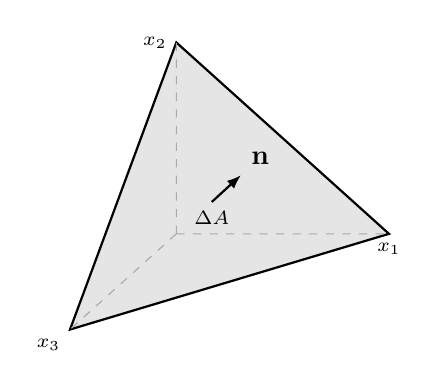
\begin{tikzpicture}[x={(1cm,0cm)},y={(0cm,1cm)},z={(-0.5cm,-0.45cm)},scale=1.35,>={Latex[length=1.8mm]}]
  \coordinate (O) at (0,0,0);
  \coordinate (X) at (2,0,0);
  \coordinate (Y) at (0,1.8,0);
  \coordinate (Z) at (0,0,2);
  \fill[LightGray!60] (X) -- (Y) -- (Z) -- cycle;
  \draw[thick] (X) -- (Y) -- (Z) -- cycle;
  \draw[dashed,DarkGray] (O) -- (X) (O) -- (Y) (O) -- (Z);
  \draw[->,thick] (0.667,0.6,0.667) -- ++(0.55,0.5,0.55) node[above right] {$\mathbf{n}$};
  \node[font=\scriptsize,below] at (0.667,0.6,0.667) {$\Delta A$};
  \node[below,font=\scriptsize] at (X) {$x_1$};
  \node[left,font=\scriptsize] at (Y) {$x_2$};
  \node[below left,font=\scriptsize] at (Z) {$x_3$};
\end{tikzpicture}

{\tiny\color{DarkGray}Schematic: instructor's course notes.\par}
\end{column}
\begin{column}{0.64\textwidth}
\footnotesize
\begin{itemize}
\item Cut a small tetrahedron with three faces normal to $-\mathbf{e}_1,-\mathbf{e}_2,-\mathbf{e}_3$ and a slanted face of area $\Delta A$ with outward normal $\mathbf{n}$. The coordinate faces have areas $\Delta A_j = n_j\,\Delta A$; the volume is $\Delta V = \tfrac13 h\,\Delta A$ ($h$ = height).
\item Linear momentum balance:
\[
\mathbf{t}(\mathbf{n})\,\Delta A + \sum_{j}\mathbf{t}(-\mathbf{e}_j)\,n_j\,\Delta A + \mathbf{b}\,\Delta V = \rho\,\mathbf{a}\,\Delta V .
\]
\item Divide by $\Delta A$ and let $h\to 0$ (volume terms vanish). With $\mathbf{t}(-\mathbf{e}) = -\mathbf{t}(\mathbf{e})$ (action--reaction):
\[
\mathbf{t}(\mathbf{n}) = \sum_j \mathbf{t}(\mathbf{e}_j)\,n_j
\ \Longrightarrow\
t_i = \sigma_{ij}\,n_j,
\]
with $\sigma_{ij} := [\mathbf{t}(\mathbf{e}_j)]_i$.
\item So the three tractions on the coordinate planes determine the traction on \emph{every} plane: this is Cauchy's theorem.
\end{itemize}
\end{column}
\end{columns}
\vspace{1mm}
{\tiny\color{DarkGray}Standard argument; see Bower (2010), \S2.2, and Gurtin, Fried \& Anand (2010).\par}
\end{frame}

\begin{frame}{Component Form of the Stress Tensor}

\begin{itemize}

\item In a Cartesian basis $\{\mathbf{e}_1,\mathbf{e}_2,\mathbf{e}_3\}$,
the components $\sigma_{ij}$ represent:
\[
\sigma_{ij} = \mathbf{e}_i \cdot (\boldsymbol{\sigma} \,\mathbf{e}_j).
\]

\item Interpretation:
\begin{itemize}
  \item $j$ = orientation of the surface normal,
  \item $i$ = direction of the traction vector.
\end{itemize}

\item Written as a matrix:
\[
\boldsymbol{\sigma}
=
\begin{bmatrix}
\sigma_{11} & \sigma_{12} & \sigma_{13} \\
\sigma_{21} & \sigma_{22} & \sigma_{23} \\
\sigma_{31} & \sigma_{32} & \sigma_{33}
\end{bmatrix}.
\]

\item Symmetry \(\sigma_{ij}=\sigma_{ji}\) follows from balance of angular momentum for a continuum without body couples or couple stresses (see the moment balance on a small cube).
\end{itemize}

\vspace{1mm}
{\tiny\color{DarkGray}Convention: with $\mathbf{t}=\boldsymbol{\sigma}\mathbf{n}$, $\sigma_{ij}$ is the $i$-component of the traction on a face with normal $\mathbf{e}_j$. Bower (2010) and many engineering texts use the transpose labelling ($\mathbf{t}=\mathbf{n}\cdot\boldsymbol{\sigma}$, first index = face); because $\boldsymbol{\sigma}$ is symmetric the numbers are identical.\par}

\end{frame}

\begin{frame}{Normal and Shear Stresses}
\begin{itemize}
\item Writing the components with coordinate labels $x,y,z$,
\[
\boldsymbol{\sigma}=
\begin{bmatrix}
\sigma_{xx} & \sigma_{xy} & \sigma_{xz}\\
\sigma_{yx} & \sigma_{yy} & \sigma_{yz}\\
\sigma_{zx} & \sigma_{zy} & \sigma_{zz}
\end{bmatrix}.
\]
\item The \textbf{diagonal} entries $\sigma_{xx},\sigma_{yy},\sigma_{zz}$ are \textbf{normal stresses}: the traction component perpendicular to the face with normal $\mathbf{e}_x$, $\mathbf{e}_y$, $\mathbf{e}_z$ (positive = tension, negative = compression).
\item The \textbf{off-diagonal} entries are \textbf{shear stresses}: traction components parallel to the face. With the convention above, $\sigma_{xy}$ is the $x$-component of the traction on the face whose normal is $\mathbf{e}_y$; by symmetry it equals $\sigma_{yx}$, the $y$-component on the face with normal $\mathbf{e}_x$.
\item This split is tied to the chosen axes: rotating the basis mixes normal and shear components. In the principal basis (eigenvectors of $\boldsymbol{\sigma}$) all shear components vanish.
\end{itemize}
\vspace{1mm}
{\tiny\color{DarkGray}Ported from the instructor's earlier notes (\texttt{OLD-2-Solid-Mechanics.tex}), with the index convention made consistent with this deck.\par}
\end{frame}

\begin{frame}{Normal and Shear Stresses on an Arbitrary Plane}
\begin{itemize}
\item On a plane with unit normal $\mathbf{n}$, the traction $\mathbf{t}=\boldsymbol{\sigma}\mathbf{n}$ splits into
\[
\sigma_n = \mathbf{n}\cdot\boldsymbol{\sigma}\mathbf{n} \quad\text{(normal stress)},\qquad
\boldsymbol{\tau} = \boldsymbol{\sigma}\mathbf{n} - \sigma_n\,\mathbf{n} \quad\text{(shear traction)},
\]
with $|\boldsymbol{\tau}|^2 = |\mathbf{t}|^2 - \sigma_n^2$.
\item Example: $\boldsymbol{\sigma}=\begin{bmatrix}2&1&0\\1&0&0\\0&0&0\end{bmatrix}\,\text{MPa}$ and $\mathbf{n}=\mathbf{e}_x$ give $\mathbf{t}=(2,1,0)$ MPa, so $\sigma_n=2$ MPa and $\boldsymbol{\tau}=(0,1,0)$ MPa.
\item A basis-independent split is into \textbf{spherical} and \textbf{deviatoric} parts:
\[
\boldsymbol{\sigma} = \underbrace{\tfrac13(\mathrm{tr}\,\boldsymbol{\sigma})\,\mathbf{I}}_{-p\,\mathbf{I}} + \boldsymbol{\sigma}', \qquad \mathrm{tr}\,\boldsymbol{\sigma}'=0,
\]
where $p=-\tfrac13\mathrm{tr}\,\boldsymbol{\sigma}$ is the mean pressure. The deviator $\boldsymbol{\sigma}'$ carries all of the shear, in every basis.
\end{itemize}
\end{frame}

\begin{frame}{Principal Stresses and Stress Invariants}
\begin{itemize}
\item Because $\boldsymbol{\sigma}$ is symmetric, it has three real eigenvalues $\sigma_1\ge\sigma_2\ge\sigma_3$ (the \textbf{principal stresses}) and an orthonormal set of eigenvectors (the \textbf{principal directions}); see the eigenvalue slides later in this deck.
\item On a plane normal to a principal direction the traction is purely normal: $\boldsymbol{\sigma}\mathbf{m}_k=\sigma_k\mathbf{m}_k$, so the shear traction is zero.
\item The largest shear traction over all planes is $\tau_{\max}=\tfrac12(\sigma_1-\sigma_3)$, on planes at $45^\circ$ to the $\mathbf{m}_1$ and $\mathbf{m}_3$ directions.
\item Invariants of stress used in practice:
\[
I_1=\mathrm{tr}\,\boldsymbol{\sigma}=\sigma_1+\sigma_2+\sigma_3=-3p,\quad
J_2=\tfrac12\,\boldsymbol{\sigma}':\boldsymbol{\sigma}',\quad
\sigma_{\rm vM}=\sqrt{3J_2}\ \text{(von Mises)} .
\]
\item Example: uniaxial tension $\sigma_{11}=\sigma_0$ (all else 0) gives $\sigma_1=\sigma_0$, $\sigma_2=\sigma_3=0$, $\tau_{\max}=\sigma_0/2$, and $\sigma_{\rm vM}=\sigma_0$.
\end{itemize}
\vspace{1mm}
{\tiny\color{DarkGray}After Bower (2010), \S2.2 (principal stresses and invariants).\par}
\end{frame}

\begin{frame}{Why the Stress Tensor Is Symmetric}

\begin{columns}[c,onlytextwidth]
\begin{column}{0.48\textwidth}
\begin{figure}[h]
    \centering
    % Native redraw of ../pictures/moment-balance-cube.jpg (JPG kept on disk; original hand sketch, source unknown).
    % Labels follow this deck's convention: sigma_{ij} = i-component of the traction on the face with normal e_j.
    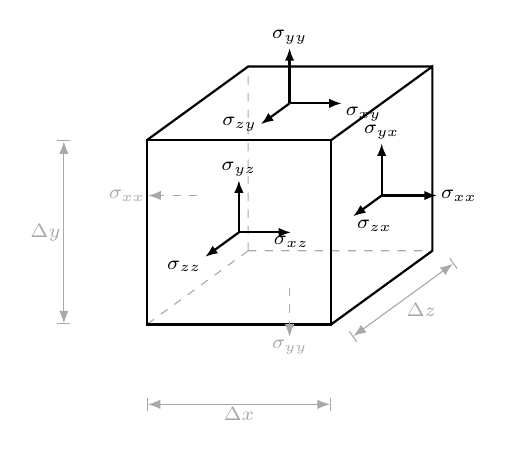
\begin{tikzpicture}[x={(1cm,0cm)},y={(0cm,1cm)},z={(-0.55cm,-0.4cm)},scale=0.78,
        >={Latex[length=1.6mm]},lab/.style={font=\scriptsize,inner sep=1pt}]
      \def\a{3}
      % hidden edges
      \draw[dashed,DarkGray] (0,0,0) -- (\a,0,0) (0,0,0) -- (0,\a,0) (0,0,0) -- (0,0,\a);
      % visible faces
      \draw[thick] (0,0,\a) -- (\a,0,\a) -- (\a,\a,\a) -- (0,\a,\a) -- cycle;
      \draw[thick] (\a,0,\a) -- (\a,0,0) -- (\a,\a,0) -- (\a,\a,\a);
      \draw[thick] (0,\a,\a) -- (0,\a,0) -- (\a,\a,0);
      % front face (normal +z)
      \draw[->,thick] (1.5,1.5,\a) -- ++(0,0,1.0) node[lab,below left] {$\sigma_{zz}$};
      \draw[->,thick] (1.5,1.5,\a) -- ++(0.85,0,0) node[lab,below] {$\sigma_{xz}$};
      \draw[->,thick] (1.5,1.5,\a) -- ++(0,0.85,0) node[lab,above] {$\sigma_{yz}$};
      % right face (normal +x)
      \draw[->,thick] (\a,1.5,1.5) -- ++(0.9,0,0) node[lab,right] {$\sigma_{xx}$};
      \draw[->,thick] (\a,1.5,1.5) -- ++(0,0.85,0) node[lab,above] {$\sigma_{yx}$};
      \draw[->,thick] (\a,1.5,1.5) -- ++(0,0,0.85) node[lab,below right] {$\sigma_{zx}$};
      % top face (normal +y)
      \draw[->,thick] (1.5,\a,1.5) -- ++(0,0.9,0) node[lab,above] {$\sigma_{yy}$};
      \draw[->,thick] (1.5,\a,1.5) -- ++(0.85,0,0) node[lab,below right] {$\sigma_{xy}$};
      \draw[->,thick] (1.5,\a,1.5) -- ++(0,0,0.85) node[lab,left] {$\sigma_{zy}$};
      % hidden faces (negative normals): equal and opposite to leading order
      \draw[->,dashed,DarkGray] (0,1.5,1.5) -- ++(-0.8,0,0) node[lab,left] {$\sigma_{xx}$};
      \draw[->,dashed,DarkGray] (1.5,0,1.5) -- ++(0,-0.8,0) node[lab,below] {$\sigma_{yy}$};
      % edge lengths
      \draw[|<->|,DarkGray] (0,-1.3,\a) -- (\a,-1.3,\a) node[midway,below,lab] {$\Delta x$};
      \draw[|<->|,DarkGray] (-1.35,0,\a) -- (-1.35,\a,\a) node[midway,left,lab] {$\Delta y$};
      \draw[|<->|,DarkGray] (\a+0.35,-0.2,\a) -- (\a+0.35,-0.2,0) node[midway,below right,lab] {$\Delta z$};
    \end{tikzpicture}
    \caption{Moment balance on a shrinking cube gives \(\sigma_{ij}=\sigma_{ji}\).}
\end{figure}
\vspace{-4mm}
{\centering\tiny\color{DarkGray}Schematic: instructor's course notes. Solid arrows: positive faces; dashed: two of the opposite (negative) faces.\par}
\end{column}
\begin{column}{0.49\textwidth}
\small
\begin{itemize}
  \item Taking moments about an axis through the centre of a cube of side \(h\), the shear tractions on opposite faces contribute a net couple proportional to \((\sigma_{ij}-\sigma_{ji})h^3\): force \(\sim \sigma h^2\) times lever arm \(\sim h\). Body \emph{forces} and rotational inertia contribute only at higher order in \(h\) (\(O(h^4)\) and \(O(h^5)\)), and so do the \(O(h)\) differences between tractions on opposite faces.
  \item A distributed body \emph{couple} (moment per unit volume) would also scale as \(h^3\); this is why it must be assumed absent.
  \item Letting \(h \to 0\) and requiring angular momentum balance therefore forces \(\sigma_{ij}=\sigma_{ji}\), provided the material transmits no body couples or couple stresses.
\end{itemize}
\end{column}
\end{columns}

\end{frame}

\begin{frame}{Why the Stress Tensor Is Symmetric: the Moment Balance in Detail}
\begin{itemize}
  \item Take moments about the $z$-axis through the centre of a cube of side $h$. Only shear tractions with a lever arm contribute:
  \begin{itemize}
    \item faces $x=\pm h/2$: traction $\pm\boldsymbol{\sigma}\mathbf{e}_x$ has $y$-component $\pm\sigma_{yx}$, force $\pm\sigma_{yx}h^2$, lever arm $\pm h/2$; together they give $+\sigma_{yx}h^3$;
    \item faces $y=\pm h/2$: traction $\pm\boldsymbol{\sigma}\mathbf{e}_y$ has $x$-component $\pm\sigma_{xy}$; using $M_z = xF_y - yF_x$ they give $-\sigma_{xy}h^3$.
  \end{itemize}
  \item Angular momentum balance about the $z$-axis:
  \[
    \underbrace{(\sigma_{yx}-\sigma_{xy})\,h^3}_{\text{surface tractions}} + \underbrace{O(h^4)}_{\text{body force, stress gradients}}
    = \underbrace{\frac{d}{dt}\big(I_{zz}\,\omega_z\big)}_{O(\rho h^5)} .
  \]
  \item Divide by $h^3$ and let $h\to 0$: $\sigma_{xy}=\sigma_{yx}$. The $x$- and $y$-axes give $\sigma_{yz}=\sigma_{zy}$ and $\sigma_{xz}=\sigma_{zx}$.
  \item In index form: $\epsilon_{ijk}\,\sigma_{kj} = 0$ for each $i$, i.e.\ $\boldsymbol{\sigma}=\boldsymbol{\sigma}^T$.
\end{itemize}
\vspace{1mm}
{\tiny\color{DarkGray}Standard argument; see Bower (2010), \S2.3 (angular momentum balance), and Gurtin, Fried \& Anand (2010).\par}
\end{frame}

\begin{frame}{The Cauchy Stress Tensor and Traction Vectors}

\textbf{Cauchy Stress Tensor.}
In continuum mechanics, the Cauchy stress tensor 
$\boldsymbol{\sigma}$ (named after Augustin–Louis Cauchy), also
called the \emph{true stress tensor}, completely characterizes
the internal state of stress at a material point in the
\emph{current} (deformed) configuration.

\medskip

\begin{itemize}
    \item It is a second–order tensor with nine components, $\sigma_{ij}.$

    \item It maps a unit direction vector $\mathbf{e}$ to the
          \textbf{traction vector} $\mathbf{T}(\mathbf{e})$ acting
          on the surface whose normal is $\mathbf{e}$:
    \[
        \mathbf{T}(\mathbf{e}) = \boldsymbol{\sigma}\,\mathbf{e},
        \qquad
        T_i(\mathbf{e}) = \sum_j \sigma_{ij} e_j.
    \]

    \item The traction vector gives the \emph{force per unit area}
          transmitted across that surface.

    \item Units: both $\boldsymbol{\sigma}$ and $\mathbf{T}$ have
          SI units of pascals (Pa). The direction vector
          $\mathbf{e}$ is dimensionless.
\end{itemize}

\vspace{1mm}
{\tiny\color{DarkGray}Text adapted from the Wikipedia article ``Cauchy stress tensor'' (CC BY-SA 4.0), \url{https://en.wikipedia.org/wiki/Cauchy_stress_tensor}.\par}

\end{frame}

\begin{frame}{Properties and Uses of the Cauchy Stress Tensor}

\begin{itemize}

    \item $\boldsymbol{\sigma}$ obeys the \textbf{tensor transformation law}:
    the components change with the coordinate system, but the physical
    traction vector $\mathbf{T}(\mathbf{e})$ does not.


    \item The Cauchy stress tensor is the appropriate stress measure for
          \textbf{small deformations} and is central in
          \textbf{linear elasticity} and most engineering stress analyses.
          (Cauchy stress is defined for \emph{any} deformation --- it is force per unit \emph{current} area; for small deformations all stress measures coincide, so it is the natural one to use there.)

    \item For \textbf{large or finite deformations}, alternative stress measures
          referred to the reference configuration are often more convenient:
    \begin{itemize}
        \item Piola–Kirchhoff stress tensors,
        \item the Biot stress tensor,
        \item the Kirchhoff stress tensor.
    \end{itemize}

    \item Despite the different forms, each of these stress measures relates
          a direction to the force transmitted across a surface—i.e., each
          is a tensor that maps vectors to vectors.

\end{itemize}

\end{frame}

\begin{frame}{Traction Vectors on an Infinitesimal Cube}

\begin{itemize}

    \item Consider a very small cube of material inside a solid.
          Each face has an outward unit normal:
          $\mathbf{e}_1$, $\mathbf{e}_2$, $\mathbf{e}_3$.

    \item The internal forces transmitted across these faces are described
          by traction vectors:
    \[
        \mathbf{T}(\mathbf{e}_1),\quad
        \mathbf{T}(\mathbf{e}_2),\quad
        \mathbf{T}(\mathbf{e}_3).
    \]

    \item By Cauchy's theorem:
    \[
        \mathbf{T}(\mathbf{e}_i) = \boldsymbol{\sigma}\,\mathbf{e}_i.
    \]

    \item Each traction vector generally contains both:
    \begin{itemize}
        \item a \textbf{normal component} (normal stress),
        \item a \textbf{tangential component} (shear stress).
    \end{itemize}

    \item Together, these tractions define the entire state of stress
          at the point—i.e., they determine the components
          $\sigma_{ij}$ of the Cauchy stress tensor.
\end{itemize}

\end{frame}

\begin{frame}{Traction Vectors and the Cauchy Stress Tensor}

\begin{figure}[h]
    \centering
    \includegraphics[width=0.75\textwidth,height=0.56\textheight,keepaspectratio]{../pictures/2-2/cauchy_stress_wiki.png}
    \caption{
        Cauchy stress tensor representation showing traction vectors on the
        faces of an infinitesimal cube (image: Wikipedia, CC BY-SA 3.0).
    }
\end{figure}
\vspace{-3mm}
{\centering\tiny\color{DarkGray}Image: Sanpaz, ``Components stress tensor cartesian.svg'', Wikimedia Commons, CC BY-SA 3.0 (\url{https://commons.wikimedia.org/wiki/File:Components_stress_tensor_cartesian.svg}). Used unmodified.\par}
\vspace{1mm}
{\tiny Note: this figure labels the components with the \emph{first} index giving the face normal and the second the direction, $\mathbf{T}^{(\mathbf{e}_i)} = \sigma_{i1}\mathbf{e}_1+\sigma_{i2}\mathbf{e}_2+\sigma_{i3}\mathbf{e}_3$, the transpose of the labelling on the previous slides. Since $\boldsymbol{\sigma}$ is symmetric the values agree.\par}

\end{frame}


\begin{frame}{Material Motion and the Deformation Gradient}

\begin{itemize}

\item Let a material point move from position $\mathbf{x}$ in the reference configuration to $\mathbf{w}(\mathbf{x})$ in the deformed configuration.
\item Consider a small material line element $d\mathbf{x}$.
\item After deformation, it becomes
\[
d\mathbf{w} = \mathbf{F}\,d\mathbf{x},
\]
where $\mathbf{F}$ is the \textbf{deformation gradient tensor}.

\item $\mathbf{F}$ describes local stretch, shear, and rotation of material fibers.
\item It is the derivative of the motion:
\[
F_{ij} = \frac{\partial w_i}{\partial x_j}.
\]

\end{itemize}

\end{frame}

\begin{frame}{Deformation Gradient Acting on Material Fibers}

\begin{itemize}
    \item Think of the body as filled with tiny material line elements (fibers).
    \item In the reference configuration, a small fiber has vector
          $d\mathbf{x}$.
    \item After deformation, that fiber becomes
          \[
              d\mathbf{w} = \mathbf{F}\,d\mathbf{x}.
          \]
    \item The deformation gradient $\mathbf{F}$:
          \begin{itemize}
              \item stretches fibers,
              \item shears them,
              \item and can rotate them.
          \end{itemize}
    \item At a point, $\mathbf{F}$ summarizes how all nearby fibers move.
\end{itemize}

\vspace{0.3cm}



\end{frame}


\begin{frame}{Why the Deformation Gradient Is a Tensor}

\begin{itemize}

\item $\mathbf{F}$ maps one vector ($d\mathbf{x}$) to another ($d\mathbf{w}$) in a linear way.
\item This mapping is purely geometric — it does not depend on the coordinate system.
\item Its components transform correctly under a basis change:
\[
F^{(m)} = Q\,F^{(e)}\,Q^T.
\]
(This assumes the same basis change is applied in the reference and deformed configurations. Strictly, $\mathbf{F}$ is a \emph{two-point} tensor: if the two bases are changed independently, $F^{\rm new} = Q_{\rm current}\,F^{\rm old}\,Q_{\rm reference}^T$.)

\item Therefore $\mathbf{F}$ is a true second-order tensor:
\begin{itemize}
  \item independent of the description,
  \item dependent only on the physical deformation.
\end{itemize}

\end{itemize}

\end{frame}

\begin{frame}{Putting It Together: Stress and Deformation Gradient}

\begin{itemize}

\item \textbf{Stress tensor} $\boldsymbol{\sigma}$: describes internal forces transmitted across surfaces.
\[
\mathbf{t} = \boldsymbol{\sigma}\,\mathbf{n}.
\]

\item \textbf{Deformation gradient} $\mathbf{F}$: describes how material line elements transform.
\[
d\mathbf{w} = \mathbf{F}\,d\mathbf{x}.
\]

\item Both objects:
\begin{itemize}
  \item map vectors to vectors,
  \item have component matrices that depend on the basis,
  \item represent physical laws independent of the coordinate system,
  \item are therefore second-order tensors.
\end{itemize}

\end{itemize}

\end{frame}

\begin{frame}{Difference Between a Matrix and a Tensor -- Part 1}

\begin{itemize}
    \item In a given basis, a second-order tensor can be represented by a
          $3 \times 3$ matrix of components.
    \item However, \emph{not every} $3 \times 3$ matrix represents a tensor.
    \item Any $3 \times 3$ matrix $[A]$ defines a rule
    \[
        \begin{bmatrix} b_1 \\[2pt] b_2 \\[2pt] b_3 \end{bmatrix}
        =
        \begin{bmatrix}
            a_{11} & a_{12} & a_{13} \\
            a_{21} & a_{22} & a_{23} \\
            a_{31} & a_{32} & a_{33}
        \end{bmatrix}
        \begin{bmatrix} u_1 \\[2pt] u_2 \\[2pt] u_3 \end{bmatrix},
    \]
    where $(u_1,u_2,u_3)$ are the components of some vector $\mathbf{u}$.
    \item The question is: does this matrix really represent a
          \emph{geometric} object (a tensor), or is it just an arbitrary
          collection of numbers?
\end{itemize}

\end{frame}

\begin{frame}{Difference Between a Matrix and a Tensor -- Part 2}

\begin{itemize}
    \item A tensor is a linear map that is \textbf{independent of the basis}.
          Its component matrix must change in a specific way when we change
          coordinates.
    \item Suppose we change to a new Cartesian basis and compute:
    \begin{itemize}
        \item the new components of $\mathbf{u}$,
        \item the new $3 \times 3$ matrix of numbers representing the same rule.
    \end{itemize}
    \item Using the new components of $\mathbf{u}$ and the new matrix,
          we obtain a new output with components $(\beta_1,\beta_2,\beta_3)$.
    \item If $(b_1,b_2,b_3)$ and $(\beta_1,\beta_2,\beta_3)$ are related by the
          \emph{same} change-of-basis rule as any other vector, then the matrix
          is behaving like the components of a vector-valued linear map.
\end{itemize}

\end{frame}

\begin{frame}{Difference Between a Matrix and a Tensor -- Part 3}

\begin{itemize}
    \item In other words: the matrix represents a \textbf{tensor} if and only if
          its components obey the \textbf{tensor transformation law}:
    \[
        S^{(m)} = Q\, S^{(e)}\, Q^{T},
    \]
    where $Q$ is the orthogonal matrix relating the two bases.
    \item If this transformation law holds, then:
    \begin{itemize}
        \item the map $\mathbf{v} = S\,\mathbf{u}$ is independent of the basis,
        \item the component triplets $(b_1,b_2,b_3)$ and $(\beta_1,\beta_2,\beta_3)$
              are just different coordinate representations of the same vector.
    \end{itemize}
    \item If the matrix does \emph{not} transform this way, it does not represent
          a genuine tensor; it is just an arbitrary matrix.
\end{itemize}
\end{frame}

\begin{frame}{Motivation: Building a Tensor from Two Directions}

\begin{itemize}

    \item A second-order tensor is a linear map that takes a vector
          $\mathbf{u}$ and produces another vector.

    \item Sometimes we want a tensor whose behavior is determined by
          \emph{two specific directions}: 
          \begin{itemize}
              \item one direction along which the output should point,
              \item another direction that controls how strongly the input
                    contributes.
          \end{itemize}

    \item The \textbf{dyadic product} provides precisely this construction.

    \item Given two vectors $\mathbf{a}$ and $\mathbf{b}$, the dyadic product
          defines a tensor $S = \mathbf{a} \otimes \mathbf{b}$ whose action on
          any vector $\mathbf{u}$ is
          \[
              S\,\mathbf{u}
              = (\mathbf{a} \otimes \mathbf{b})\,\mathbf{u}
              = \mathbf{a}\,(\mathbf{b} \cdot \mathbf{u}).
          \]
          \end{itemize}
\end{frame}

\begin{frame}{Motivation: Building a Tensor from Two Directions (cont.)}
\begin{itemize}
    \item Interpretation:
          \begin{itemize}
              \item First, measure how much of $\mathbf{u}$ lies in direction
                    $\mathbf{b}$ (the scalar projection $\mathbf{b}\cdot\mathbf{u}$).
              \item Then, scale the vector $\mathbf{a}$ by that amount.
          \end{itemize}

    \item The result is always a vector \emph{parallel to $\mathbf{a}$}, with
          magnitude depending on the component of $\mathbf{u}$ in the
          direction of $\mathbf{b}$.

\end{itemize}

\end{frame}

\begin{frame}{Components of a Dyadic Product and Tensor Construction}

\begin{itemize}

    \item In a Cartesian basis $\{\mathbf{e}_1,\mathbf{e}_2,\mathbf{e}_3\}$,
          the components of $S = \mathbf{a} \otimes \mathbf{b}$ are simply
          outer products of the components of $\mathbf{a}$ and $\mathbf{b}$:
          \[
              S_{ij} = a_i\, b_j.
          \]

    \item In matrix form:
          \[
          \begin{bmatrix}
              a_1 b_1 & a_1 b_2 & a_1 b_3 \\
              a_2 b_1 & a_2 b_2 & a_2 b_3 \\
              a_3 b_1 & a_3 b_2 & a_3 b_3
          \end{bmatrix}.
          \]

    \item A single dyadic product cannot represent an arbitrary tensor,
          because $S\,\mathbf{u}$ is always parallel to $\mathbf{a}$.
          So the mapping is too restrictive.
    \end{itemize}
\end{frame}


\begin{frame}{Components of a Dyadic Product and Tensor Construction (cont.)}

\begin{itemize}
    \item However, dyadic products form a natural \emph{basis} for all
          second-order tensors.

    \item If $\mathbf{e}_1,\mathbf{e}_2,\mathbf{e}_3$ is a basis, then the nine
          dyads
          \[
              \mathbf{e}_i \otimes \mathbf{e}_j
          \]
          form a basis for the space of all $3\times 3$ tensors.

    \item Therefore, \textbf{any} second-order tensor can be written as a sum of
          dyadic products:
          \[
              S = \sum_{i=1}^{3} \sum_{j=1}^{3} S_{ij}\,
                  \mathbf{e}_i \otimes \mathbf{e}_j.
          \]
          This expresses the tensor in terms of simple “direction-pair”
          building blocks.

\end{itemize}

\end{frame}

\begin{frame}{Worked Example: A Dyadic (Tensor) Product}
\begin{columns}[T,onlytextwidth]
\begin{column}{0.48\textwidth}
\begin{itemize}
\item Take
\[
\mathbf{a} = \begin{bmatrix} 1 \\ 2 \\ 3 \end{bmatrix}, \qquad
\mathbf{b} = \begin{bmatrix} 4 \\ 5 \\ 6 \end{bmatrix}.
\]
\item $S=\mathbf{a}\otimes\mathbf{b}$ has components $S_{ij}=a_i b_j$: row $i$ is $a_i$ times the whole (row) vector $\mathbf{b}^T$:
\[
\begin{aligned}
\text{row 1}: &\; 1\cdot(4,5,6) = (4,5,6)\\
\text{row 2}: &\; 2\cdot(4,5,6) = (8,10,12)\\
\text{row 3}: &\; 3\cdot(4,5,6) = (12,15,18)
\end{aligned}
\]
\end{itemize}
\end{column}
\begin{column}{0.50\textwidth}
\begin{itemize}
\item Hence
\[
\mathbf{a}\otimes\mathbf{b} = \mathbf{a}\,\mathbf{b}^T =
\begin{bmatrix} 4 & 5 & 6 \\ 8 & 10 & 12 \\ 12 & 15 & 18 \end{bmatrix}.
\]
\item Check the defining action on $\mathbf{u}=\mathbf{e}_1$: $(\mathbf{a}\otimes\mathbf{b})\mathbf{e}_1 = \mathbf{a}\,(\mathbf{b}\cdot\mathbf{e}_1) = 4\mathbf{a} = (4,8,12)^T$, the first column. \checkmark
\end{itemize}
\end{column}
\end{columns}
\vspace{1mm}
{\tiny\color{DarkGray}Ported from the instructor's earlier notes (\texttt{OLD-2-Solid-Mechanics.tex}).\par}
\end{frame}

\begin{frame}{Worked Example: A Dyadic Product (continued)}
\begin{itemize}
\item Every column of $\mathbf{a}\otimes\mathbf{b}$ is a multiple of $\mathbf{a}=(1,2,3)^T$ (column $j$ is $b_j\mathbf{a}$), so the matrix has \textbf{rank one} and $\det(\mathbf{a}\otimes\mathbf{b})=0$. This is the matrix form of ``$S\mathbf{u}$ is always parallel to $\mathbf{a}$''.
\item Order matters: $\mathbf{b}\otimes\mathbf{a} = (\mathbf{a}\otimes\mathbf{b})^T = \begin{bmatrix} 4 & 8 & 12 \\ 5 & 10 & 15 \\ 6 & 12 & 18 \end{bmatrix}$.
\item The trace is the dot product: $\mathrm{tr}(\mathbf{a}\otimes\mathbf{b}) = 4+10+18 = 32 = \mathbf{a}\cdot\mathbf{b}$.
\item The tensor product generalizes to higher order: if $\mathbf{A}$ has order $m$ and $\mathbf{B}$ has order $n$, then $(\mathbf{A}\otimes\mathbf{B})_{i_1\dots i_m j_1\dots j_n} = A_{i_1\dots i_m}B_{j_1\dots j_n}$ has order $m+n$ (e.g.\ the stiffness tensor $C_{ijkl}$ is fourth order).
\end{itemize}
\end{frame}


\begin{frame}{Representing Tensor Components with Matrices (recap)}
    {\footnotesize\color{DarkGray}Recap of ``Matrix Representation of a Tensor'' above; it opens the tensor-algebra reference section that follows Bower, Appendix B.\par}
    \begin{itemize}
        \item   Second-order tensors can be represented by matrices.

        \item   Consider a general second-order tensor \( \mathbf{S} \).

        \item   In a given basis, we can express \(\mathbf{S}\) using its components \(S_{ij}\) arranged in a 3x3 matrix:

            \[
            \mathbf{S} =
            \begin{bmatrix}
                S_{11} & S_{12} & S_{13} \\
                S_{21} & S_{22} & S_{23} \\
                S_{31} & S_{32} & S_{33}
            \end{bmatrix}
            \]

        \item   Here, \(i\) and \(j\) each range from 1 to 3 in 3-dimensional space.

        \item   The values of the components \(S_{ij}\) depend on the choice of basis.

        \item   This matrix representation allows us to apply matrix operations (addition, multiplication, etc.) to tensors.
    \end{itemize}
\end{frame}

\begin{frame}
\frametitle{Defining Individual Tensor Components (recap of the dyadic form)}
\begin{itemize}
    \item Where the individual components are defined as: 
    \begin{align*}
        S_{11} &= e_1 \cdot (S e_1), & S_{12} &= e_1 \cdot (S e_2), & S_{13} &= e_1 \cdot (S e_3) \\
        S_{21} &= e_2 \cdot (S e_1), & S_{22} &= e_2 \cdot (S e_2), & S_{23} &= e_2 \cdot (S e_3) \\
        S_{31} &= e_3 \cdot (S e_1), & S_{32} &= e_3 \cdot (S e_2), & S_{33} &= e_3 \cdot (S e_3)
    \end{align*}
    \item The tensor representation can also use dyadic form:
    \[
    S = \sum_{i=1}^{3} \sum_{j=1}^{3} S_{ij} e_i \otimes e_j
    \]
    \item This is useful for polar coordinates.
    \item (Why: in polar or other curvilinear coordinates the basis vectors $\mathbf{e}_r,\mathbf{e}_\theta$ vary from point to point, so it is safest to keep the basis dyads $\mathbf{e}_i\otimes\mathbf{e}_j$ explicit when differentiating; Bower, Appendix D.)
\end{itemize}
\end{frame}

\begin{frame}
\frametitle{Adding Second Order Tensors}
\begin{itemize}
    \item If S and T are tensors, then \(U = S + T\) is also a tensor. 
    \item If the Cartesian components of U, S, and T are defined by matrices, then: 
    \[
    \begin{bmatrix}
        U_{11} & U_{12} & U_{13} \\
        U_{21} & U_{22} & U_{23} \\
        U_{31} & U_{32} & U_{33}
    \end{bmatrix} =
    \begin{bmatrix}
        S_{11} + T_{11} & S_{12} + T_{12} & S_{13} + T_{13} \\
        S_{21} + T_{21} & S_{22} + T_{22} & S_{23} + T_{23} \\
        S_{31} + T_{31} & S_{32} + T_{32} & S_{33} + T_{33}
    \end{bmatrix}
    \]
\end{itemize}
\end{frame}

\begin{frame}
\frametitle{Product of a Tensor and a Vector}
\begin{itemize}
    \item Let u be a vector and S a second order tensor.  Then
    \[
    v = S u
    \]
    is a vector. 
    \item Let \((u_1, u_2, u_3)\) and \((v_1, v_2, v_3)\) be the components of vectors u and v, and let the Cartesian components of S be defined as above. 
    \item Then
    \[
    \begin{bmatrix}
        v_1 \\
        v_2 \\
        v_3
    \end{bmatrix} =
    \begin{bmatrix}
        S_{11} & S_{12} & S_{13} \\
        S_{21} & S_{22} & S_{23} \\
        S_{31} & S_{32} & S_{33}
    \end{bmatrix}
    \begin{bmatrix}
        u_1 \\
        u_2 \\
        u_3
    \end{bmatrix} =
    \begin{bmatrix}
        S_{11} u_1 + S_{12} u_2 + S_{13}u_3 \\
        S_{21} u_1 + S_{22} u_2 + S_{23}u_3 \\
        S_{31} u_1 + S_{32} u_2 + S_{33}u_3
    \end{bmatrix}
    \]
\end{itemize}
\end{frame}

\begin{frame}
\frametitle{Product of a Vector and a Tensor}
\begin{itemize}
    \item Let $\mathbf{u}$ be a vector and $S$ a second-order tensor. Then
    \[
      \mathbf{v} = \mathbf{u} S
    \]
    is also a vector.
    \item In component form (with respect to a Cartesian basis):
    \[
      v_i = \sum_{j=1}^3 u_j\, S_{ji}, \qquad i = 1,2,3.
    \]
    \item In matrix notation:
    \[
      \begin{bmatrix} v_1 & v_2 & v_3 \end{bmatrix}
      =
      \begin{bmatrix} u_1 & u_2 & u_3 \end{bmatrix}
      \begin{bmatrix}
        S_{11} & S_{12} & S_{13} \\
        S_{21} & S_{22} & S_{23} \\
        S_{31} & S_{32} & S_{33}
      \end{bmatrix}.
    \]
    \item In general, $\mathbf{u} S \neq S \mathbf{u}$ (unless $S$ is symmetric).
\end{itemize}
\end{frame}


\begin{frame}
\frametitle{Product of Two Tensors}
\small
\begin{itemize}
    \item Let $T$ and $S$ be second–order tensors. Then $U = TS$ is also a tensor.
    \item Write the components of $U$, $T$, and $S$ as $3\times 3$ matrices:
\[
U =
\begin{bmatrix}
U_{11} & U_{12} & U_{13} \\
U_{21} & U_{22} & U_{23} \\
U_{31} & U_{32} & U_{33}
\end{bmatrix}
=
\begin{bmatrix}
T_{11} & T_{12} & T_{13} \\
T_{21} & T_{22} & T_{23} \\
T_{31} & T_{32} & T_{33}
\end{bmatrix}
\begin{bmatrix}
S_{11} & S_{12} & S_{13} \\
S_{21} & S_{22} & S_{23} \\
S_{31} & S_{32} & S_{33}
\end{bmatrix}
\]

\vspace{-2mm}
\scriptsize
\[
= \begin{bmatrix}
T_{11}S_{11} + T_{12}S_{21} + T_{13}S_{31} &
T_{11}S_{12} + T_{12}S_{22} + T_{13}S_{32} &
T_{11}S_{13} + T_{12}S_{23} + T_{13}S_{33} \\
T_{21}S_{11} + T_{22}S_{21} + T_{23}S_{31} &
T_{21}S_{12} + T_{22}S_{22} + T_{23}S_{32} &
T_{21}S_{13} + T_{22}S_{23} + T_{23}S_{33} \\
T_{31}S_{11} + T_{32}S_{21} + T_{33}S_{31} &
T_{31}S_{12} + T_{32}S_{22} + T_{33}S_{32} &
T_{31}S_{13} + T_{32}S_{23} + T_{33}S_{33}
\end{bmatrix}
\]
\small
    \item Tensor products are not commutative: $TS \neq ST$.
\end{itemize}
\end{frame}


\begin{frame}
\frametitle{Tensor Transpose}
\begin{itemize}
    \item Let S be a tensor. The transpose of S, denoted by \(S^T\), is defined such that
    \[
    u S^T = S u
    \]
    \item If the components of S are defined by a 3x3 matrix, then the components of \(S^T\) are: 
    \[
    S^T =
    \begin{bmatrix}
        S_{11} & S_{21} & S_{31} \\
        S_{12} & S_{22} & S_{32} \\
        S_{13} & S_{23} & S_{33}
    \end{bmatrix}
    \]
    i.e., the rows and columns are interchanged. 
    \item For tensors A and B: 
    \[
    (A B)^T = B^T A^T
    \]
\end{itemize}
\end{frame}

\begin{frame}
\frametitle{Tensor Trace}
\begin{itemize}
    \item Let S be a tensor with components defined by a \(3 \times 3\) matrix. 
    \item The trace of S, denoted by tr(S) or trace(S), is the sum of the diagonal elements: 
    \[
    trace(S) = S_{11} + S_{22} + S_{33}
    \]
    \item For any Cartesian basis \(\{e_1, e_2, e_3\}\):
    \[
    trace(S) = e_1 \cdot (S e_1) + e_2 \cdot (S e_2) + e_3 \cdot (S e_3)
    \]
    \item The trace of a tensor is invariant under a change of basis. 
\end{itemize}
\end{frame}

\begin{frame}
\frametitle{Tensor Contraction: Inner Product}
\begin{itemize}
    \item Let S and T be two second order tensors. 
    \item The inner product of S and T is a scalar, denoted by \(S : T\). 
    \item Using components of S and T in a basis: 
    \[
    S : T = S_{11}T_{11} + S_{12}T_{12} + S_{13}T_{13}
    \]
    \[
    + S_{21}T_{21} + S_{22}T_{22} + S_{23}T_{23}
    \]
    \[
    + S_{31}T_{31} + S_{32}T_{32} + S_{33}T_{33}
    \]
    \item Note that \(S : T = T : S\) and \(S : I = trace(S)\) where I is the identity tensor. 
\end{itemize}
\end{frame}

\begin{frame}
\frametitle{Tensor Contraction: Outer Product}
\begin{itemize}
    \item Let S and T be two second order tensors. 
    \item The outer product of S and T is a scalar, denoted by \(S \cdot \cdot T\). 
    \item Using components of S and T in a basis:
    \[
    S \cdot \cdot T = S_{11}T_{11} + S_{21}T_{12} + S_{31}T_{13}
    \]
    \[
    + S_{12}T_{21} + S_{22}T_{22} + S_{32}T_{23}
    \]
    \[
    + S_{13}T_{31} + S_{23}T_{32} + S_{33}T_{33}
    \]
    \item Note that \(S \cdot \cdot T = S^T : T\)
    \item Compactly, \(S : T = S_{ij}T_{ij}\) and \(S\cdot\cdot T = S_{ij}T_{ji} = \mathrm{tr}(ST)\) (sum over repeated indices). For symmetric \(S\) or \(T\) the two coincide.
    \item Naming caution: Bower calls \(S\cdot\cdot T\) the ``outer product'', but it is a \emph{scalar} (a double contraction). It is not the tensor (dyadic) product \(S\otimes T\), which is a fourth-order tensor.
\end{itemize}
\end{frame}

\begin{frame}
\frametitle{Tensor Determinant}
\begin{itemize}
    \item The determinant of a tensor is the determinant of its component matrix in a basis. 
    \item For a second order tensor: 
    \[
    det S = det
    \begin{bmatrix}
        S_{11} & S_{12} & S_{13} \\
        S_{21} & S_{22} & S_{23} \\
        S_{31} & S_{32} & S_{33}
    \end{bmatrix}
    \]
    \small
    \[
    = S_{11}(S_{22}S_{33} - S_{23}S_{32}) + S_{12}(S_{23}S_{31} - S_{21}S_{33}) + S_{13}(S_{21}S_{32} - S_{31}S_{22})
    \]

    \item For tensors S and T: 
    \[
    det(S) = det(S^T)
    \]
    \[
    det(S T) = det(S)det(T)
    \]
\end{itemize}
\end{frame}

\begin{frame}
\frametitle{Tensor Inverse}
\begin{itemize}
    \item Let S be a second order tensor. 
    \item The inverse of S, denoted by \(S^{-1}\), exists if and only if \(det(S) \neq 0\), and is defined by: 
    \[
    S^{-1} S = I
    \]
    where I is the identity tensor.
    \item The inverse can be computed from the inverse of the component matrix. 
    \item A compact form for a general 3D second order tensor is complex, and methods like Gaussian elimination are preferred. 
\end{itemize}
\end{frame}

\begin{frame}
\frametitle{Tensor Eigenvalues and Eigenvectors}
\begin{itemize}
    \item The scalars \(\lambda\) and unit vectors m which satisfy
    \[
    S m = \lambda m
    \]
    are known as the eigenvalues and eigenvectors of S, or the principal values and principal directions of S.
    \item Note that \(\lambda\) may be complex.
    \item For a second order tensor in three dimensions, there are generally three values of \(\lambda\) and three unit vectors m (each determined up to sign) which satisfy this equation.
\end{itemize}
\end{frame}

\begin{frame}
\frametitle{Tensor Eigenvalues and Eigenvectors (continued)}
\begin{itemize}
    \item Occasionally, there may be only two or one distinct value of \(\lambda\). For a symmetric tensor, a repeated eigenvalue means there are infinitely many possible vectors m that satisfy the equation, spanning an eigenplane or all of space. (A non-symmetric tensor with a repeated eigenvalue may instead be defective, with fewer independent eigenvectors than eigenvalues.)
    \item The eigenvalues of a tensor, and the components of the eigenvectors, may be computed by finding the eigenvalues and eigenvectors of the matrix of components.
    \item The eigenvalues of a symmetric tensor are always real.
    \item The eigenvalues of a skew tensor are always pure imaginary or zero.
\end{itemize}
\end{frame}

\begin{frame}
\frametitle{Change of Basis}
{\footnotesize\color{DarkGray}Recap of the tensor transformation law stated earlier, now with a proof.\par}
\begin{itemize}
    \item Let S be a tensor, and let \(\{e_1, e_2, e_3\}\) be a Cartesian basis.
    \item Suppose that the components of S in the basis \(\{e_1, e_2, e_3\}\) are known to be
    \[
    [S^{(e)}] =
    \begin{bmatrix}
        S_{11}^{(e)} & S_{12}^{(e)} & S_{13}^{(e)} \\
        S_{21}^{(e)} & S_{22}^{(e)} & S_{23}^{(e)} \\
        S_{31}^{(e)} & S_{32}^{(e)} & S_{33}^{(e)}
    \end{bmatrix}
    \]
\end{itemize}
\end{frame}

\begin{frame}
\frametitle{Change of Basis (continued)}
\begin{itemize}
    \item Now, suppose that we wish to compute the components of S in a second Cartesian basis, \(\{m_1, m_2, m_3\}\). Denote these components by
    \[
    [S^{(m)}] =
    \begin{bmatrix}
        S_{11}^{(m)} & S_{12}^{(m)} & S_{13}^{(m)} \\
        S_{21}^{(m)} & S_{22}^{(m)} & S_{23}^{(m)} \\
        S_{31}^{(m)} & S_{32}^{(m)} & S_{33}^{(m)}
    \end{bmatrix}
    \]
\end{itemize}
\end{frame}

\begin{frame}
\frametitle{Change of Basis: Transformation Matrix}
\begin{itemize}
    \item To do so, first compute the components of the transformation matrix [Q]
    \[
    [Q] =
    \begin{bmatrix}
        m_1 \cdot e_1 & m_1 \cdot e_2 & m_1 \cdot e_3 \\
        m_2 \cdot e_1 & m_2 \cdot e_2 & m_2 \cdot e_3 \\
        m_3 \cdot e_1 & m_3 \cdot e_2 & m_3 \cdot e_3
    \end{bmatrix}
    \]
    (this is the same matrix you would use to transform vector components from \(\{e_1, e_2, e_3\}\) to \(\{m_1, m_2, m_3\}\)).
\end{itemize}
\end{frame}

\begin{frame}
\frametitle{Change of Basis: Tensor Transformation}
\begin{itemize}
    \item Then,
    \[
    [S^{(m)}] = [Q] [S^{(e)}] [Q]^T
    \]
    or, written out in full
    \scriptsize
    \begin{multline*}
    \begin{bmatrix}
        S_{11}^{(m)} & S_{12}^{(m)} & S_{13}^{(m)} \\
        S_{21}^{(m)} & S_{22}^{(m)} & S_{23}^{(m)} \\
        S_{31}^{(m)} & S_{32}^{(m)} & S_{33}^{(m)}
    \end{bmatrix} =
    \\
    \begin{bmatrix}
        m_1 \cdot e_1 & m_1 \cdot e_2 & m_1 \cdot e_3 \\
        m_2 \cdot e_1 & m_2 \cdot e_2 & m_2 \cdot e_3 \\
        m_3 \cdot e_1 & m_3 \cdot e_2 & m_3 \cdot e_3
    \end{bmatrix}
    \begin{bmatrix}
        S_{11}^{(e)} & S_{12}^{(e)} & S_{13}^{(e)} \\
        S_{21}^{(e)} & S_{22}^{(e)} & S_{23}^{(e)} \\
        S_{31}^{(e)} & S_{32}^{(e)} & S_{33}^{(e)}
    \end{bmatrix}
    \begin{bmatrix}
        m_1 \cdot e_1 & m_2 \cdot e_1 & m_3 \cdot e_1 \\
        m_1 \cdot e_2 & m_2 \cdot e_2 & m_3 \cdot e_2 \\
        m_1 \cdot e_3 & m_2 \cdot e_3 & m_3 \cdot e_3
    \end{bmatrix}
    \end{multline*}
\end{itemize}
\end{frame}

\begin{frame}
\frametitle{Change of Basis: Proof}
\begin{itemize}
    \item To prove this result, let u and v be vectors satisfying
    \[
    v = S u
    \]
    \item Denote the components of u and v in the two bases by \(u^{(e)}\), \(v^{(e)}\) and \(u^{(m)}\), \(v^{(m)}\) respectively.
    \item Recall that the vector components are related by
    \[
    u^{(m)} = [Q] u^{(e)} \qquad u^{(e)} = [Q]^T u^{(m)}
    \]
    \[
    v^{(m)} = [Q] v^{(e)} \qquad v^{(e)} = [Q]^T v^{(m)}
    \]
\end{itemize}
\end{frame}

\begin{frame}
\frametitle{Change of Basis: Proof (continued)}
\begin{itemize}
    \item Now, we could express the tensor-vector product in either basis
    \[
    v^{(m)} = [S^{(m)}] u^{(m)}
    \]
    \[
    v^{(e)} = [S^{(e)}] u^{(e)}
    \]
    \item Substitute for \(u^{(e)}\) and \(v^{(e)}\) from above into the second of these two relations, we see that
    \[
    [Q]^T v^{(m)} = [S^{(e)}] [Q]^T u^{(m)}
    \]
\end{itemize}
\end{frame}

\begin{frame}
\frametitle{Change of Basis: Proof (end)}
\begin{itemize}
    \item Recall that
    \[
    [Q] [Q]^T = [I]
    \]
    \item so multiplying both sides by [Q] shows that
    \[
    v^{(m)} = [Q] [S^{(e)}] [Q]^T u^{(m)}
    \]
    \item Since this must hold for every $u^{(m)}$, the matrix acting on $u^{(m)}$ must be $[S^{(m)}]$, so
    \[
    [S^{(m)}] = [Q] [S^{(e)}] [Q]^T
    \]
    as stated.
\end{itemize}
\end{frame}

\begin{frame}
\frametitle{Invariants}
\begin{itemize}
    \item Invariants of a tensor are functions of the tensor components which remain constant under a basis change.
    \item That is to say, the invariant has the same value when computed in two arbitrary bases \(\{e_1, e_2, e_3\}\) and \(\{m_1, m_2, m_3\}\).
    \item A symmetric second order tensor always has three independent invariants.
\end{itemize}
\end{frame}

\begin{frame}
\frametitle{Examples of Invariants}
\begin{itemize}
    \item The standard set is the three \emph{principal invariants}
    \begin{enumerate}
        \item \(I_1 = \mathrm{tr}\,S\)
        \item \(I_2 = \tfrac{1}{2}\left[(\mathrm{tr}\,S)^2 - \mathrm{tr}(S^2)\right]\)
        \item \(I_3 = \det S\)
    \end{enumerate}
    \item These are the coefficients of the characteristic polynomial, so they are exactly the symmetric functions of the three eigenvalues.
    \item Other quantities—the eigenvalues themselves, the trace, the determinant, and the inner and outer products—are invariants too, but they are not independent of \(I_1, I_2, I_3\): any of them can be computed from the eigenvalues, and the eigenvalues from \(I_1, I_2, I_3\).
    \item (This holds for symmetric \(S\), as assumed on the previous slide. For example \(S\cdot\cdot S = \mathrm{tr}(S^2) = I_1^2 - 2I_2\) always, and \(S:S = \mathrm{tr}(S^TS)\) equals it when \(S=S^T\). For a non-symmetric \(S\), \(S:S\) is an additional invariant not determined by the eigenvalues.)
    \item Characteristic polynomial: \(\det(S-\lambda I) = -\lambda^3 + I_1\lambda^2 - I_2\lambda + I_3\), so \(I_1=\lambda_1+\lambda_2+\lambda_3\), \(I_2=\lambda_1\lambda_2+\lambda_2\lambda_3+\lambda_3\lambda_1\), \(I_3=\lambda_1\lambda_2\lambda_3\).
\end{itemize}
\end{frame}

\begin{frame}
\frametitle{Special Tensors: Identity Tensor}
\begin{itemize}
    \item The identity tensor I is the tensor such that, for any tensor S or vector v
    \[
    I v = v I = v
    \]
    \[
    S I = I S = S
    \]
    \item In any basis, the identity tensor has components
    \[
    \begin{bmatrix}
        1 & 0 & 0 \\
        0 & 1 & 0 \\
        0 & 0 & 1
    \end{bmatrix}
    \]
\end{itemize}
\end{frame}

\begin{frame}
\frametitle{Special Tensors: Symmetric Tensor}
\begin{itemize}
    \item A symmetric tensor S has the property
    \[
    S = S^T
    \]
    \item The components of a symmetric tensor have the form
    \[
    \begin{bmatrix}
        S_{11} & S_{12} & S_{13} \\
        S_{12} & S_{22} & S_{23} \\
        S_{13} & S_{23} & S_{33}
    \end{bmatrix}
    \]
    so that there are only six independent components of the tensor, instead of nine.
\end{itemize}
\end{frame}

\begin{frame}
\frametitle{Special Tensors: Skew Tensor}
\begin{itemize}
    \item A skew tensor S has the property
    \[
    S^T = -S
    \]
    \item The components of a skew tensor have the form
    \[
    \begin{bmatrix}
        0 & S_{12} & S_{13} \\
        -S_{12} & 0 & S_{23} \\
        -S_{13} & -S_{23} & 0
    \end{bmatrix}
    \]
\end{itemize}
\end{frame}

\begin{frame}
\frametitle{Special Tensors: Orthogonal Tensors}
\begin{itemize}
    \item An orthogonal tensor S has the property
    \[
    S S^T = S^T S = I
    \]
    \[
    S^{-1} = S^T
    \]
    \item An orthogonal tensor must have \(det(S) = \pm 1\). A tensor with \(det(S) = +1\) is known as a proper orthogonal tensor.
\end{itemize}
\end{frame}

\begin{frame}
\frametitle{Attribution}
Sections on tensor algebra are adapted from A. F. Bower, \emph{Applied Mechanics of Solids}
(CRC Press, 2010), Appendix B, whose online version at \url{http://solidmechanics.org}
is made freely available for non-commercial educational use. Used here for teaching.

\medskip
The stress slides draw on Bower (2010), \S2.2--2.3, and on the Wikipedia article ``Cauchy stress tensor''. The worked dyadic-product example and the normal/shear decomposition are ported from the instructor's earlier notes (\texttt{OLD-2-Solid-Mechanics.tex}).
\end{frame}

\begin{frame}{References}
\scriptsize
\begin{itemize}
  \item A. F. Bower, \emph{Applied Mechanics of Solids}, CRC Press, Boca Raton, 2010. doi:10.1201/9781439802489. Online: \url{https://solidmechanics.org} (Appendix B: tensors; Appendix D: polar coordinates; \S2.2--2.3: stress and its symmetry).
  \item M. E. Gurtin, E. Fried, L. Anand, \emph{The Mechanics and Thermodynamics of Continua}, Cambridge University Press, 2010. doi:10.1017/CBO9780511762956 (tensor algebra; Cauchy's theorem; symmetry of stress).
  \item Wikipedia contributors, ``Cauchy stress tensor'', \emph{Wikipedia}, CC BY-SA 4.0, \url{https://en.wikipedia.org/wiki/Cauchy_stress_tensor}.
  \item Sanpaz, ``Components stress tensor cartesian.svg'', Wikimedia Commons, CC BY-SA 3.0, \url{https://commons.wikimedia.org/wiki/File:Components_stress_tensor_cartesian.svg}.
  \item Instructor's earlier notes, \texttt{OLD-2-Solid-Mechanics.tex} (worked dyadic example; normal and shear stresses).
\end{itemize}
\medskip
\textbf{Figures.} Stress cube for the symmetry argument: schematic redrawn for these notes (earlier sketch \texttt{pictures/moment-balance-cube.jpg} kept on disk).

\medskip
\textbf{Further reading.} G. A. Holzapfel, \emph{Nonlinear Solid Mechanics}, Wiley, 2000, Ch.~1 (vectors and tensors); P. A. Kelly, \emph{Solid Mechanics Part III}, University of Auckland lecture notes (online), Ch.~1 (vectors and tensors).
\end{frame}
\end{document}
